%%%%%%%%%%%%%%%%%%%%%%%%%%%%%%%%%%%%%%%%%
% baposter Landscape Poster
% LaTeX Template
% Version 1.0 (11/06/13)
%
% baposter Class Created by:
% Brian Amberg (baposter@brian-amberg.de)
%
% This template has been downloaded from:
% http://www.LaTeXTemplates.com
%
% License:
% CC BY-NC-SA 3.0 (http://creativecommons.org/licenses/by-nc-sa/3.0/)
%
%%%%%%%%%%%%%%%%%%%%%%%%%%%%%%%%%%%%%%%%%

%----------------------------------------------------------------------------------------
%	PACKAGES AND OTHER DOCUMENT CONFIGURATIONS
%----------------------------------------------------------------------------------------

\documentclass[landscape,a0paper,fontscale=0.285]{baposter} % Adjust the font scale/size here
\usepackage{url}
\usepackage{bm}
\usepackage{graphicx} % Required for including images
\graphicspath{{figures/}} % Directory in which figures are stored

\usepackage{amsmath} % For typesetting math
\usepackage{amssymb} % Adds new symbols to be used in math mode

\usepackage{booktabs} % Top and bottom rules for tables
\usepackage{enumitem} % Used to reduce itemize/enumerate spacing
\usepackage{palatino} % Use the Palatino font
\usepackage[font=small,labelfont=bf]{caption} % Required for specifying captions to tables and figures

\usepackage{multicol} % Required for multiple columns
\setlength{\columnsep}{1.5em} % Slightly increase the space between columns
\setlength{\columnseprule}{0mm} % No horizontal rule between columns

\usepackage{tikz} % Required for flow chart
\usetikzlibrary{shapes,arrows} % Tikz libraries required for the flow chart in the template

\newcommand{\compresslist}{ % Define a command to reduce spacing within itemize/enumerate environments, this is used right after \begin{itemize} or \begin{enumerate}
\setlength{\itemsep}{1pt}
\setlength{\parskip}{0pt}
\setlength{\parsep}{0pt}
}

\definecolor{lightblue}{rgb}{0.145,0.6666,1} % Defines the color used for content box headers

\begin{document}

\begin{poster}
{
headerborder=closed, % Adds a border around the header of content boxes
colspacing=1em, % Column spacing
bgColorOne=gray, % Background color for the gradient on the left side of the poster
bgColorTwo=white, % Background color for the gradient on the right side of the poster
borderColor=black, % Border color
headerColorOne=black, % Background color for the header in the content boxes (left side)
headerColorTwo=orange, % Background color for the header in the content boxes (right side)
headerFontColor=white, % Text color for the header text in the content boxes
boxColorOne=white, % Background color of the content boxes
textborder=roundedleft, % Format of the border around content boxes, can be: none, bars, coils, triangles, rectangle, rounded, roundedsmall, roundedright or faded
eyecatcher=true, % Set to false for ignoring the left logo in the title and move the title left
headerheight=0.1\textheight, % Height of the header
headershape=roundedright, % Specify the rounded corner in the content box headers, can be: rectangle, small-rounded, roundedright, roundedleft or rounded
headerfont=\Large\bf\textsc, % Large, bold and sans serif font in the headers of content boxes
%textfont={\setlength{\parindent}{1.5em}}, % Uncomment for paragraph indentation
linewidth=2pt % Width of the border lines around content boxes
}
%----------------------------------------------------------------------------------------
%	TITLE SECTION 
%----------------------------------------------------------------------------------------
%
{
\includegraphics[height=4em]{PS_HOR_RGB_2C.png}} % First university/lab logo on the left
{\bf\textsc{The Network of Foreign Direct Investment Flows}\vspace{0.5em}} % Poster title
{\textsc{J. Schoeneman, B. Zhu, \& B. Desmarais\\
Pennsylvania State University}} % Author names and institution
{
{\includegraphics[height=4em]{nsf.png}} % Second nsf logo on the right
{
\includegraphics[height=4em]{bdss.png}}
}
%----------------------------------------------------------------------------------------
%	introduction
%----------------------------------------------------------------------------------------

\headerbox{Introduction}{name=objectives,column=0,row=0}{

The political economy of FDI literature has established several theoretical claims and empirical regularities regarding exogenous political and economic determinants of FDI inflows.  However, existing studies---based on monadic and to a lesser degree, dyadic regression models---overlook the complex dependencies that are likely to characterize the network. Recent developments in methodology for studying international relations show that the regression framework is typically inadequate for quantitatively modeling dyadic relational data, such as FDI flows. In this paper, we integrate hypotheses regarding exogenous determinants and novel hypotheses regarding structural dependencies into a comprehensive exponential random graph model (ERGM) for weighted networks.

\vspace{0.3em} % When there are two boxes, some whitespace may need to be added if the one on the right has more content
}

%----------------------------------------------------------------------------------------
%	Theory
%----------------------------------------------------------------------------------------

\headerbox{Theory}{name=introduction,column=1,row=0,bottomaligned=objectives}{
MNC expansion via FDI often face opposition from host countries due to concerns over national security and protection for local firms that do not want to compete with foreign firms. To overcome this political opposition, countries enter into reciprocal agreements. Therefore we expect one structural dependency to be mutuality, which we measure as the increase of FDI given the minimum value in the dyad.\\
The second structural dependency we model is transitivity, or the likelihood that country A, will send FDI to country C, given that country A sends FDI to country B and country B send FDI to country C. We expect this clustering given the fragmented global supply chains for production and the vertical FDI that follows. 

}

%----------------------------------------------------------------------------------------
%	RESULTS
%----------------------------------------------------------------------------------------

\headerbox{Key Results}{name=results,column=2,span=2,row=0}{

\centering
\begin{tabular}{c@{\hskip -.4cm}c@{\hskip -.4cm}c}
Log-GDP Product & Distance  & PTA Depth  \\
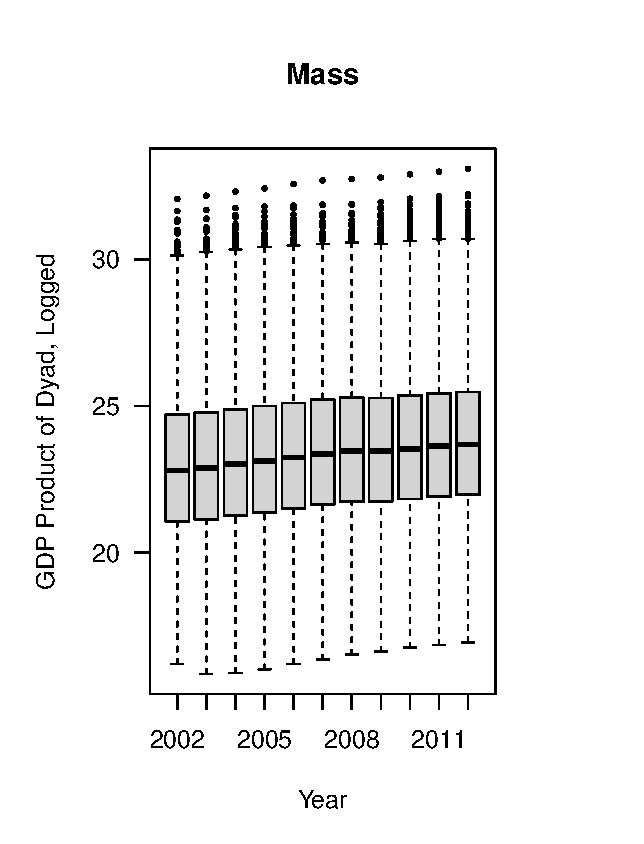
\includegraphics[height=.14\textheight, clip=true, trim=0cm .5cm 0cm .1cm]{figures/rl_plots/mass.pdf}    &
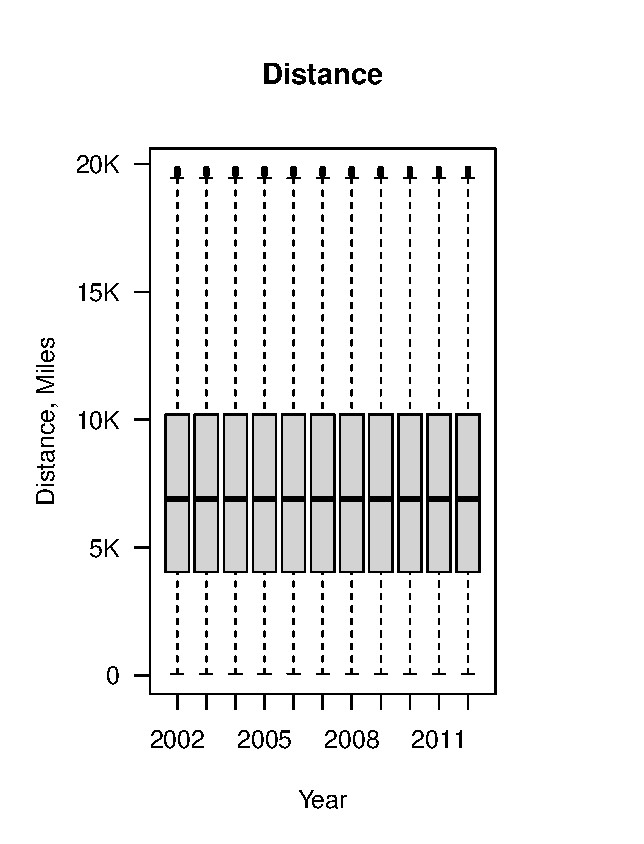
\includegraphics[height=.14\textheight, clip=true, trim=.5cm .5cm 0cm .1cm]{figures/rl_plots/distance.pdf}   &
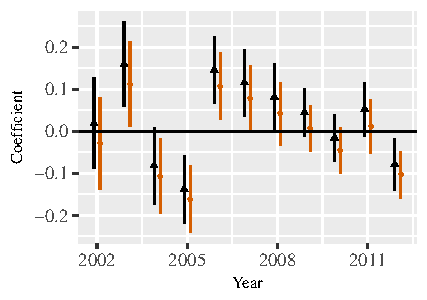
\includegraphics[height=.14\textheight, clip=true, trim=.5cm .5cm 0cm .1cm]{figures/rl_plots/PTADepth.pdf}\\


Destination Polity & Mutuality & Transitivity \\ 
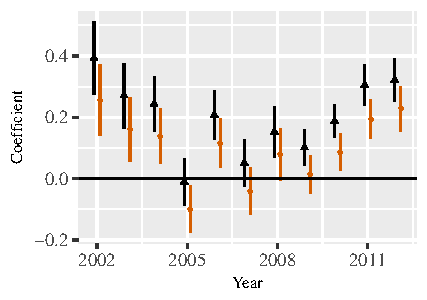
\includegraphics[height=.14\textheight, clip=true, trim=0cm .5cm 0cm .1cm]{figures/rl_plots/DestPolity.pdf} 
 &
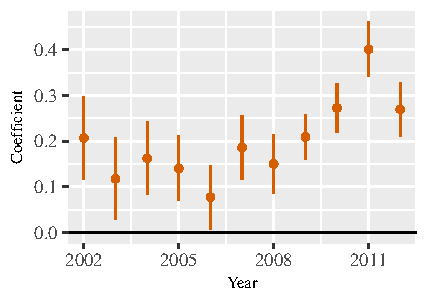
\includegraphics[height=.14\textheight, clip=true, trim=.5cm .5cm 0cm .1cm]{figures/rl_plots/Mutuality.pdf}   &
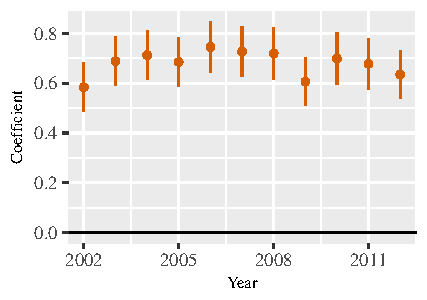
\includegraphics[height=.14\textheight, clip=true, trim=.5cm .5cm 0cm .1cm]{figures/rl_plots/Transitivity.pdf} \\  
\end{tabular}
\vfill
Bars represents 95\% Confidence intervals. Black triangles are estimates without controlling for network dependencies, Orange circles are estimates with network controls.

}

%----------------------------------------------------------------------------------------
%	Acknowledgement
%----------------------------------------------------------------------------------------

\headerbox{Acknowledgement}{name=references,column=0,above=bottom}{

This material is based on work supported by the National Science Foundation under IGERT Grant DGE-1144860, Big Data Social Science.}

%----------------------------------------------------------------------------------------
%	REFERENCES
%----------------------------------------------------------------------------------------

\headerbox{References}{name=futureresearch,column=1,span=2,aligned=references,above=bottom}{ % This block is as tall as the references block


\small{1. D{\"u}r, A., Baccini, L., \& Elsig, M. (2014). The design of international trade agreements: Introducing a new dataset. The Review of International Organizations, 9(3), 353-375.}

}

%----------------------------------------------------------------------------------------
%	CONTACT INFORMATION
%----------------------------------------------------------------------------------------

\headerbox{Contact Information}{name=contact,column=3,aligned=references,above=bottom}{ % This block is as tall as the references block

\begin{description}\compresslist
\item[Web] \url{https://github.com/desmarais-lab/FDI_IGERT_H}
\item[Email] jbs5686@psu.edu
\end{description}
}

%----------------------------------------------------------------------------------------
%	Network Plot
%----------------------------------------------------------------------------------------

\headerbox{Network Plots}{name=conclusion,column=2,span=2,row=0,below=results,above=references}{

\begin{multicols}{2}
\begin{center}
\captionof{figure}{Plot for 2011. Blue represents autocratic regimes and red represents democratic regimes}
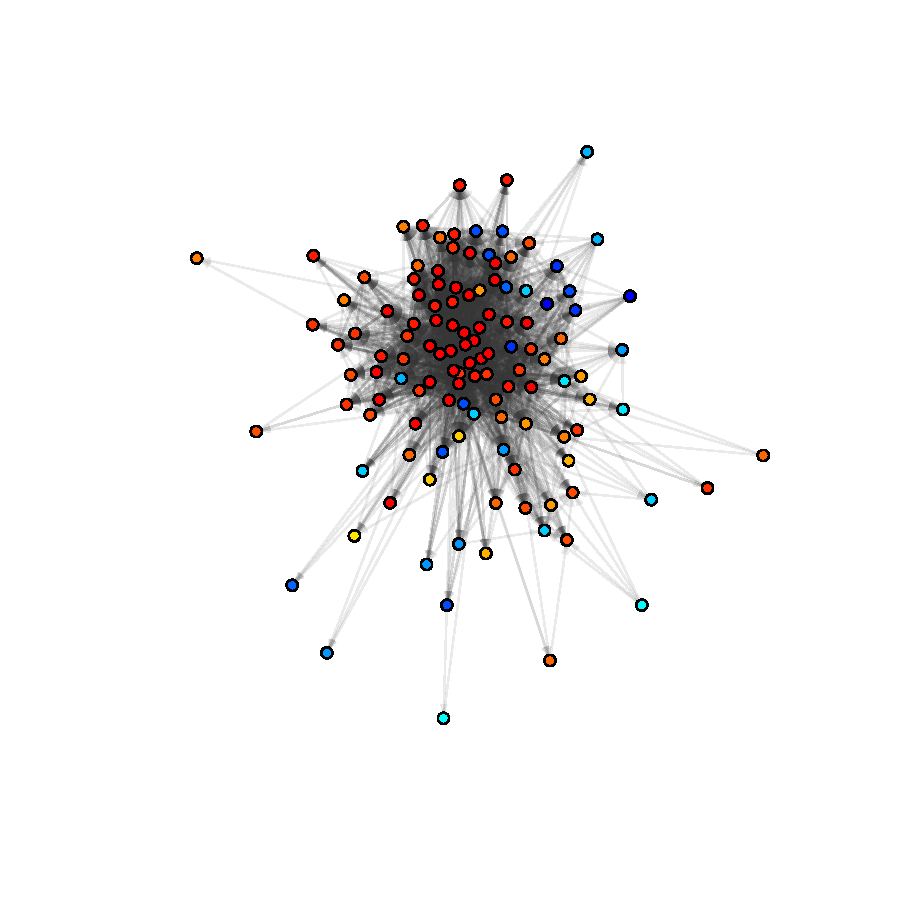
\includegraphics[width=0.8\linewidth]{fdiNet2011.pdf}
\end{center}

%------------------------------------------------

\begin{itemize}\compresslist


\item{Clustering, based on the edges between nodes, which here is FDI flow between countries, is visually present.} 

\item{ It also appears that regime type plays a role in clustering as well, with red, democratic nodes often close to one another, albeit weakly. This assortativity is measured below.} 

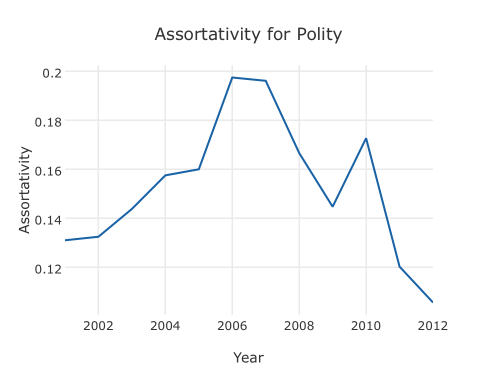
\includegraphics[scale= .3]{assortativity.png}

\end{itemize}

\end{multicols}
}

%----------------------------------------------------------------------------------------
% Data and Software
%----------------------------------------------------------------------------------------

\headerbox{Data}{name=method,column=0,below=objectives,bottomaligned=conclusion}{ % This block's bottom aligns with the bottom of the conclusion block

\begin{itemize}\compresslist
\item{Bilateral FDI statistics from UNCTAD, 2001-2012}
\item{Dyad-level Covariates}
\begin{itemize}
\item{Gravity +} 
\item{Contiguity +} 
\item{Common Language +} 
\item{Four Types of Defense Treaties +}  
\item{Colonial Relationships +}
 \item{PTA depth$^{1}$ + }
\end{itemize}
\item{Node-level Covariates}
\begin{itemize}
\item{GDP per capita +/-} 
\item{GDP Growth Rate +} 
\item {Polity IV +} 
\item{Political Violence - } 
\item{Trade Openness +}
\end{itemize}
\end{itemize}
}

%----------------------------------------------------------------------------------------
%	Count Model
%----------------------------------------------------------------------------------------

\headerbox{ERGM Count Model}{name=results2,column=1,below=objectives,bottomaligned=conclusion}{ % This block's bottom aligns with the bottom of the conclusion block
$ \text{Pr}_{\bm{\theta};h;\bm{g}}( \bm{Y}=\bm{y} )=\frac{ h(\bm{y})\text{exp}( \bm{\theta} \cdot \bm{g} (\bm{y}) )}{\bm{\kappa}_{h,\bm{g}}(\bm{\theta})} $\\

$\text{Sum}:\bm{g(y)} = \sum_{(i,j) {\in} \mathbb{Y}}\bm{y}_{i,j}$\\

$\text{Sum, Fractional Moment}:\bm{g(y)} = \sum_{(i,j) {\in} \mathbb{Y}}\bm{y}_{i,j}^{1/2}$\\

$\text{Non-Zero}: \bm{g}_k = \sum_{(i,j) {\in} \mathbb{Y}} \mathbb{I}(\bm{y}_{i,j} \neq 0)$\\

$ \text{Reciprocity}: \bm{g(y)} = \sum_{(i,j) {\in} \mathbb{Y}}min(\bm{y}_{i,j},\bm{y}_{j,i})$\\

$\text{Transitive Weights}: \\\bm{g(y)} =  \sum_{(i,j) {\in} \mathbb{Y}}\min\bigg( \bm{y}_{i,j}, \max\limits_{k{\in}N}\Big(\min(\bm{y}_{i,k},\bm{y}_{k,j})\Big) \bigg),$\\ 

$ \text{Dyadic Covariate}: \bm{g(y,x)} = \sum_{(i,j)} \bm{y}_{i,j}x_{i,j}$ \\

$ \text{Sender Covariate}: \bm{g(y,x)} = \sum_{i}x_i \sum_{j} \bm{y}_{i,j}$\\

$ \text{Receiver Covariate}: \bm{g(y,x)} = \sum_{j}x_j \sum_{i} \bm{y}_{i,j}$\\


}

%----------------------------------------------------------------------------------------




\end{poster}

\end{document}